
\documentclass[conference]{IEEEtran}


\usepackage{listings}
\usepackage{epsfig}
\usepackage{url}
\usepackage{cite}
\usepackage{fancybox}
\usepackage{amsthm}

\newcommand{\tana}{\textsc{TANA}}

\begin{document}

\title{TANA: Fined-grained Side-channel Inforamtion Leakage Quantifications in Binaries}
\author{Anonymous}

\maketitle

\begin{abstract}
Side-channel attacks allow attackers to infer some sensitive information based on 
non-functional characteristics. Existing works on address-base side-channel detection 
can provide a list of potential side-channels leakage sites. We observed that those 
works still have the following limitations: 1) Many software may have multiple information 
leakage sites. Some vulnerabilities could be more severe than others. But existing work 
couldn’t tell the difference between those leakages. 2)  An attacker could exploit multiple 
leakages at one time. However, no existing tool can report how much information is leaked 
in total.

To overcome the above limitations: we proposed a tool called TANA, which can not only 
find the side channels but can estimate how many bits are actually leaked through the 
leakage. TANA works in three phases. First, the application is executed to record the 
trace. Second, TANA runs the instruction level symbolic execution on the top of the 
execution trace. Tana will find side-channel information leakages and model each leakage 
as one unique math constraints. Finally, TANA will classify those constraints into 
independent multiple groups and run the multiple step monte carlo to estimate the 
information leakage. TANA will a very fined-grained result compared to existing tools. 

We apply the tool on OpenSSL, MbedTLS and libjpeg and find several serious side channel 
vulnerabilities. We also evaluate the vulnerabilities from previous research. The result 
indicates most of the reported vulnerabilities are actually hard to exploit in practice.

\end{abstract}

\IEEEpeerreviewmaketitle
\pagenumbering{arabic}

\section{Introduction}
%% side channels are important
Side channels are inevitable in modern computer systems as the sensitive information 
may be leaked by many kinds of inadvertent behaviors, 
such as power, electromagnetic radiation and even 
sound~\cite{agrawal2002side,kar20178,chari1999towards,217605,genkin2014rsa}. 
Among them, software-based side channels, such as cache attacks, memory page attacks,
and controlled-channel attacks, are especially common 
and have been studied for years~\cite{7163052, 217543, 217589, lee2017inferring, 191010}. 
These vulnerabilities result from vulnerable software and shared hardware components.
By observing the outputs or hardware behaviors, attackers can
infer the program execution flow that manipulate secrets and 
guess the secrets such as encryption keys~\cite{Osvik2006}.

%% to deal with side channels, we can protect or detect them and detection is better
Various countermeasures have been proposed to defend against 
software-based side-channel attacks. Hardware level solutions, 
including reducing shared resources, adopting oblivious RAM, and using
transnational memory~\cite{203878,217537} need new hardware features or changes
to modern complex computer systems, which is impractical and hard to adopt in 
reality. Therefore, a more promising and universal direction is software countermeasures, 
detecting and eliminating side channel vulnerabilities from code.

Regarding the root cause of software-based side channels, 
many of them are caused by the following two specific types: 
data flow from secrets to load addresses and data flow from secrets to branch conditions.
We call them secret-dependent control-flow and memory-access correspondingly.
Therefore, a central problem is identifying those two code patterns automatically.
Recent works~\cite{203878,217537,Wichelmann:2018:MFF:3274694.3274741,Brotzman19Casym,236338,182946} 
adopt static and dynamic analysis
to detect side-channels.
They can find many potential leak sites in real-world software, 
but fail to report how severe a potential leakage could be. 
Many of the reported vulnerabilities are typically hard to exploit
and leak very little information. For example, DATA~\cite{217537} reports
2,246 potential leakage site for the RSA implementation in OpenSSL\@.
After some inspections, 1,510 are dismissed, but it still
leaves 278 control-flow and 460 data-access patterns. For software
developers, it is hard for them to fix all those vulnerabilities,
let alone the majority of them are negligible.
While some vulnerabilities can be used to recover the full secret
keys~\cite{184415}, many other vulnerabilities prove to be less serious in reality.

To assess the sensitive level of side-channel vulnerabilities, we need a proper 
quantification metric.
Static methods~\cite{182946,5207642}, usually with abstract interpretations, can give a leakage upper bound, 
which is useful to justify the implementation is secure when they report zero or little leakage. 
However, they cannot indicate how serious the leakage is because of over-approximation. 
For example, CacheAudit~\cite{182946} reports that the upper bound leakage of AES-128 exceeds 
the original key size! The dynamic methods take another approach with a concrete input and 
run the program in real environment. Although they are very precise in term of true leakages, 
no existing tool can precisely assess the severity of the vulnerabilities they discover.

To overcome these limitations, we propose a novel method
to quantify information leakage more precisely. 
Different from previous works, which only consider the
``average'' information leakage, we study the problem based on real attack scenarios.
The average information assumes that the target program will have \emph{variable}
or \emph{random} sensitive 
information when an attack is launched.
However, for real-world attacks, an adversary may run the target problem again and over again 
with \emph{fixed} unknown sensitive information such as the key. 
Therefore, the previous threat model cannot model real attack scenarios.
In contrast, our method is more precise and fine-grained. 
We quantify the amount of leaked information as the cardinality of the set of 
possible inputs based on attackers' observations. 

Before an attack, an adversary has a big but finite input space.
Every time when the adversary observes a leakage site, he can eliminate some 
potential inputs and reduce the size of the input space. 
The smaller the input space is, the more information is actually gained. 
In an extreme case, if the size of the input space reduces to one, 
the adversary can determine the input information uniquely, which means all the secret information
(e.g., the whole secret key) is leaked. By counting the number of distinct inputs, 
we can quantify the information leakage more precisely. 

We use constraints to model the relation between the original sensitive input and
each leakage site. We run the instruction level symbolic execution on the whole
execution trace to generate the constraints. Symbolic execution can provide the fine-grained
information but is usually believed to be an expensive operation in terms of performance. 
Therefore, existing dynamic symbolic execution based works~\cite{203878,236338,Brotzman19Casym} 
either only analyze 
small programs or apply some domain knowledge to simplify the execution. We systematically
analyze the bottleneck of the symbolic execution and optimize it scalable to
real-world crypto systems. 

We apply the above technique and build a tool called \tool{}, 
  %\footnote{CleverHans is a horse that can ``count''.
  %Our tool uses an advanced method to count the number of leaked bits from side channels.}
which can discover potential information leakage sites 
as well as estimating how many bits they can leak for each leakage site. 
We assume that adversaries can exploit secret-dependent control-flow transfers and 
data-access patterns when the program processes different sensitive data. 
%We refer them as the potential information leakage sites. 
First, we collect the dynamic execution trace for each input of the target libraries 
and then run symbolic execution on the traces. 
In this way, we model each side-channel leakage as a math formula. 
The sensitive input is divided into several independent bytes and each byte is regarded as 
a unique symbol. Those formulas can precisely model side-channel vulnerabilities.
Then we extend the problem to multiple leakages and related leakages
and introduce a monte carlo sampling method to estimate the single and combined information leakage.
In fact, if an application has a different sensitive input but still satisfies the formula, 
the code can still leak the same information. 


%Based on the fixed attack target, we classify the software-based side-channel 
%vulnerabilities into two categories: 1.\textit{secret-dependent control-flow transfers} 
%and 2.\textit{secret-dependent data accesses} and model them with math formulas which
%constrain the value of sensitive information.
%We quantify the amount of leaked information as the number of possible solutions that are
%reduced after applying each constrains.


%Our method can identify and quantify address-based
%sensitive information leakage sites in real-world applications automatically. 
%Adversaries can exploit different control-flow transfers and data-access patterns when 
%the program processes different sensitive data. We refer them as the potential information
%leakage sites. Our tool can discover and estimate those potential information leakage sites 
%as well as how many bits they can leak. We are also able to report precisely how many bits
%can be leaked in total if an attacker observes more than one site.
%We run symbolic execution on execution traces. We model each side-channel leakage as a math formula. 
%The sensitive input is divided into several independent bytes and each byte is regarded as 
%a unique symbol. Those formulas can precisely model every the side-channel vulnerability. 
%In other words, if the application has a different sensitive input but still satisfies the formula, 
%the code can still leak the same information.  
%Those information leakage sites may spread in the whole program 
%and their leakages may not be dependent. Simply adding them up can only get a coarse upper bound 
%estimate. In order to accurately calculate the total information leakage, we must know the 
%dependent relationships among those multiple leakages sites. Therefore, we introduce a 
%monte carlo sampling method to estimate the total information leakage.

We apply \tool{} on both symmetric and asymmetric ciphers from
real-world crypto libraries including OpenSSL and mbed TLS\@. The
experimental result confirms that \tool{} can precisely identify the
previous known vulnerabilities, report how much information is leaked
and which byte in the original sensitive buffer is leaked.  Although
some of the analyzed crypto libraries have a number of side-channels,
they actually leak very little information. Also, we perform the
analysis of widely deployed software countermeasures against side
channels.  \tool\ also discovers new vulnerabilities. With the help of
\tool{}, we confirm those vulnerabilities can be exploited.

In summary, we make the following contributions:

\begin{itemize}
  \item We propose a novel method that can quantify fine-grained
    leaked information from side-channel vulnerabilities to match real
    attack scenarios.  Our method is different from previous ones in
    that we model real attack scenarios more precisely while the
    previous research only models the ``average'' or ``random'' case.
    Our results are surprisingly different,
    % compared to previous results and
    much more useful in practice.
    %%   We model each side-channel vulnerabilities as math formulas
    %% and mutiple side-channel vulnerabilities can be seen as the
    %% conjunction of those formulas, which precisely models the
    %% program semantics.
        
  \item We transfer the information quantification problem into a
    counting problem and use the Monte Carlo sampling
    method to estimate the information leakage. Some initial results
    indicate the the sampling method suffers from the curse of
    dimensionality problem. We therefore design a guided sampling
    method and provide the corresponding error estimate.
        
  \item We implement the proposed method into a practical tool and
    apply it on several real-world software. \tool{} successfully
    identifies memory-related side-channel vulnerabilities and
    provides the corresponding information leakage. The information
    leakage result provides the detailed information that can help
    developers to fix the reported vulnerabilities.
\end{itemize}

\section{Background}
In this section, we first present an introduction to software-based 
side-channel attacks. These attacks are what we study in the paper. 
After that, we will discuss existing methods on side-channel detection 
and quantification.

\subsection{Software-based Side-Channels}
Side-channels are information channels that can 
leak sensitive information unconsciously through different 
behaviors.  

Fundamentally, those differences were caused by the memory 
hierarchy design in modern computer systems. When a CPU 
fetches data, it first searches
the cache, which stores copies of data that was frequently 
referred in main memory. If the data does not exist in the cache, 
the CPU will read the data from the main memory (RAM). 

\subsubsection{Cache-based Attacks}
In general, the cached-based side-channels rely on the time differences 
between the cache miss
and the cache hit. Here we introduce two frequently used cache attacks:
PRIME+PROBE and FLUSH+RELOAD.

\textit{PRIME+PROBE} targets a single cache set. It has two phases. During the
``prime'' phase, the attacker fills the cache set with his data.
In the second ``probe'' phase, the attacker re-accesses the cache set
again. If the victim accesses the cache set and evicts part of 
the data, the attacker will experience a slow measurement. If not, 
it will be fast. By knowing which cache set the target
program accesses, the attacker can infer locations of
the sensitive information.

\textit{FLUSH+RELOAD} targets a single cache line. 
It requires the attacker and victim share the same memory.
It also has two phases. During the ``flush'' stage, the attacker 
flushes the ``monitored memory'' from the cache. Then the attacker
waits for the victim to access the memory. In the next phase, the 
attacker reload the ``monitored memory''. If the time is short, which
indicates there is a cache hit and the victim loaded the memory before. 
On the other hand, the time will be longer since the CPU need to reload
the memory into the cache line. 

\subsubsection{Memory-based Attack}
Memory-based side-channel attack~\cite{7163052} exploits the different behaviors when the
program accesses different page tables. For example, the controlled-channel attack~\cite{7163052},
which works in the kernel space, can infer the sensitive data in the shielding systems by
observing the page fault sequences after restricting some code and
data pages. 

After examining the memory-based side-channels attack, we believe the root
cause of those attacks are secret-dependent memory access and control
flow transfers.  \fixme{This paragraph is confusing. Secret-dependent memory access and control
  flow transfers can be cache-based side channels. We need further develop this so it is not a surprise
when it is mentioned in the next subsection. It is better to classify these into 'branch-taken-related' and 'data-accessed-related.'}

%
%\lstinputlisting[language=c, 
%                 numbers=left,
%                 caption={Sample code shows secret-dependent memory access and 
%                          secret-dependent control-flow transfer.},
%                 captionpos=b,
%                 label={code:background},
%                 frame=single,
%                 basicstyle=\fontsize{7}{9}\selectfont\ttfamily]
%                 {sample_code/background.c}

%For example, the above code~\ref{code:background} show a simple encryption function that
%has the two kinds of side-channels. At line 11, depending on the value of a key,
%the code will access the different entry in the predefined table. At the
%line 13, the code will do a series of computation and determine if the code in the if
%branch is executed or not. Such vulnerabilities are called the memory-based 
%side-channles. We identify and quantify the leakage of the two kinds of vulnerabilities 
%in the paper.

\subsection{Information Leakage Quantification}

\fixme{Section (II.B), this subsection: Clarify mutual information, min-entropy, and maximal leakage. How many types? maybe use subsubsection}

Given an event $e$ which occurs with the probability $P(e)$, if the event $e$ happens, 
then we receive
\begin{displaymath}
    I = - \log_2P(e)
\end{displaymath}
bits of information by knowing the event $e$.
Consider a char variable $a$ in a C program, which has the size
of one byte (8 bits). It ranges from 0 -- 255.  Assume
 \textit{a} has the uniform distribution. If at one time we observe that $a$
equals $1$, the probability of this observation is $\frac{1}{256}$. So the information we get is 
$-\log(\frac{1}{256}) = 8$ bits, which is exactly the size of the char variable in the C program.

Some existing work on information leakage quantification is based on mutual information or 
min-entropy \cite{10.1007/978-3-642-00596-1_21}.
In these frameworks, the input sensitive
information $K$ is viewed as a random variable. Let $k_i$ be one of the possible
value of $K$. The Shannon entropy $H(K)$ is defined as
\begin{displaymath}
    H(K) = - \sum_{k_i {\in} K}P(k_i)\log_2P(k_i)
\end{displaymath}

The Shannon entropy can be used to quantify the initial uncertainty about the sensitive
information. Suppose a program with some
sensitive input $K$, an adversary has some observations ($O$) through some side channel.
In this work, the observations are referred as the secret-dependent control-flows and
secret-dependent data-access patterns. \fixme{See the comment above, we need to explain these
  patterns before this point.} The conditional entropy $H(K|O)$ is
\begin{displaymath}
    H(K|O) = - \sum_{o_j {\in} O} {P(o_j) \sum_{k_i {\in} K}{P(k_i|o_j)\log_2P(k_i|o_j)}}
\end{displaymath}
Intuitively, the conditional information marks the uncertainty about $K$ after the adversary
has gained some observations ($O$). 

Some previous work uses the mutual information $I(K; O)$ to quantify the leakage which is defined 
as follows:
\begin{displaymath}
    \mathit{Leakage} = I(K;O) = \sum_{k_i {\in} K}{\sum_{o_j {\in} O}{P(k_i, o_j)\log_2\frac{P(k_i, o_j)}{P(k_i)P(o_j)}}}
\end{displaymath}
where $P(k_i, o_i)$ is the joint discrete distribution of $K$ and $O$.
Alternatively, the mutual information can also be computed with the following equation:
\begin{displaymath}
    \mathit{Leakage} = I(K;O) = H(K) - H(K|O) = H(O) - H(O|K)
\end{displaymath}

For a deterministic program, once the input $K$ is fixed, the program will have the same
control-flow transfers and data-access patterns. As a result, $P(k_i, o_j)$ will always
equals to 1 or 0. So the conditional entropy $H(O|K)$ will equal to zero. So the leakage defined
by the mutual information can be simplified into:
\begin{displaymath}
\label{mutual:information}
    \mathit{Leakage} = I(K;O) = H(O)
\end{displaymath}
In other words, once we know the distribution of those memory-access patterns. We can 
calculate how much information is actually leaked.

Another common method is based on the maximal leakage~\cite{10.1007/978-3-642-00596-1_21,10.1007/978-3-642-31424-7_40,182946}.
The formal information theory can prove that the maximal leakage is the upper bound of the mutual 
information (Channel Capacity).

\begin{displaymath}
    \mathit{Leakage} = \log(C(O))
\end{displaymath}
Here $C(O)$ represents the number of different observations that an attacker can have. 

%% put this example in next section
%%\section{Running Example}

%Now we provide a concrete example to show how the two types of quantification definition works and show that
%how our method is different.

%\vspace{3pt}
%\textbf{Maximal Leakage.} 
%Depending on the value of key, the code can run four different branches which corrosponding to 
%four different observations. Therefore, by the maximal leakage definition, the leakage equals to 
%$\log4 = 2$ bits.

%\vspace{3pt}
%\textbf{Mutual Information.}
%If the key satisfies the uniform distribution, the probability of the code runs each branch
%can be computed with the following result.  

%\begin{table}[h]
%\centering
%\resizebox{\columnwidth}{!}{
%\begin{tabular}{|c|c|c|c|c|}
%\hline
%Branch & A     & B      & C      & D       \\ \hline
%Possibility      & 1/256 & 64/256 & 64/256 & 127/256 \\ \hline
%\end{tabular}
%}
%\caption{The distribution of observations}
%\end{table}

%Therefore, the leakage equals to 
%$\frac{1}{256}\log\frac{1}{256} + \frac{1}{4}\log\frac{1}{4}*2 + \frac{127}{256}\log\frac{127}{256} = 1.7$ bits.

%\vspace{3pt}
%\textbf{\tool.}
%\fixme{What is out result here? Need explain}

\section{Threat Model}
We consider an attacker who shares the same hardware resource with the victim. 
The attacker attempt to retrieve sensitive information via memory-based side-channel attack. 
The attacker has no direct access to the memory or cache, but can probe the memory 
or cache at each program point. Similar to DATA, the attacker will face many 
noisy observations or can only observe a limited of memory or caches in practice. 
For the project, we assume the attacker can have noise-free observations. 
This threat model captures most of the cache-based and memory-based side channel attacks.

\section{Chanllenges}

In this section, we articulate several chanllenges and existing problems
in quantifying the side-channel vulnerability leakages. We briefly describe the
chanllenges and then present the corresponding solutions.

\subsection{Information Leakage Definition}
Existing static-based side-channel quantification works defined information leakage
as the mutual information or the max leakage. Those definitions provide strong security guarantee
when trying to show a program is secure if the their methods say the program leaks zero bits of
information.

However, the above definition is less useful when if the program has some leakages. 
Considering the example in section~\ref{code::entropy}, if an attacker observes the
code runs branch A, the attacker can know the key actually equals to 128. Suppose it is 
a dummy password checker, in which case the attacker can fully retrieve the password.
Therefore, the total information leakage should be 8 bits, which equals to the size
of unsigned char. 
According to the mutual definition, however, the leakage will be 1.7 bits. The maximal information
leakage is 2 bits. Both approaches fail to precisely tell how much information is actually leaked
during the exectution.

The problem with the existing method is that they are static-based and the sensitive
input values are neglected. They assume the attacker runs the program multiple times 
with many different sensitive information as the input. Both the mutual information 
and the max-leakage give an ``average" estimate of the information leakage. 
But it isn't the typical scenario for an adversary to launch the side-channel attack.
When a side-channel attack happens, the adversary wants to retrieve the sensitive
information. So it is very likely that the sensitive input is fixed (e.g. AES keys). 
The adversary will run the attack over and over again and guesses bit by bit. Like the 
previous example, the existing static method doesn’t work well in those situations.

In the project, we hope to give a very precise definition of information leakages. 
Suppose an attacker run the target program mutiple times with one fixed input, we
want to how much information he can infer by oberserving the memory access patterns.
We come to the simple slogan ~\cite{10.1007/978-3-642-00596-1_21} where the information
leakage equals:

\textit{initial uncertainty - remaining uncertainty}

If an adversary has zero knowledge about the input before the attack. The initial uncertainty
equals to the size the input. As for the remaining uncertainty, we come to the original definition
of the information content.

Solutioin: We quantify the information leakage with the following definition. 

\newtheorem{mydef}{Definition}

\begin{mydef}
\label{def}
Given a program $P$ with the input set $K$, 
an adversary has the observation $o$ when the input $k{\in}K$. 
We denote it as
    $$P(k) = o$$
The leakage $L_{Pko}$ based on the oberservation is
    $$L_{Pko} = log_2{|K|} - log_2{|K^o|}$$
    where
    $$K^o = \{k^{'} | k^{'}{\in}K \ and \ P(k^{'}) = o \}$$
\end{mydef}

With the new definition, if the attacker observes the branch 1 was executed, then the
$K^{o^{1}} = \{128\}$. Therefore, the information leakage $L_{Pko^{1}} = log_2{256} - log_2{1} = 8$
bits, which means the key is totally leaked. If the attacker observes the code runs other
branches, the leaked information is shown in the following table.

\begin{table}[h]
    \centering
    \begin{tabular}{|c|c|c|c|c|}
    \hline
    Branch & 1 & 2  & 3  & 4   \\ \hline
    $K^o$   & 1 & 64 & 64 & 127 \\ \hline
    $L_{Pko}$(bits)   & 8 & 2  & 2  & 1   \\ \hline
    \end{tabular}
    \caption{The leaked information by the definition}
\end{table}

\subsection{Multiple Leak Sites}
Real-world software can have various side-channel vulnerabilities. Those vulnerabilities 
may spread in the whole program. An adversary may exploit more than one side-channel vulnerabilities 
to gain more information~\cite{7163052, 191010}. For example, the controlled-side channel attack~\cite{7163052}, the author 
demonstrates an attack against a popular spell checking tool, Hunspell. By observing four sets 
of secret-dependent memory accesses sites in two functions $HashMgr::addword$ and $HashMgr::lookup$, 
the author can recover the word that Hunspell checks.

For the Hunspell, the attacker manually studies the source code of Hunspell, figure out
the relation of those vulnerabilities and launch the attack. In order to precisely quantify the
total information leakage, we need to know the relation of those leakage sites. 

\lstinputlisting[language=c, 
                 numbers=left,
                 numbersep=5pt,                   % how far the line-numbers are from the code
                 caption={Multiple leakages},
                 %frame = simple,
                 captionpos=b,
                 label={code::multiple},
                 basicstyle=\fontsize{7}{9}\selectfont\ttfamily]
                 {sample_code/motivation_multiple.c}

Considering the running example in ~\ref{code::multiple}, in which $k1$, $k2$ and $k3$ are
the sensitive key. The code has six different leakage. Leakage 1, 2, 3 are the secret-dependent
data accesses and leakage 4, 5, 6 are the secret-dependent control-flow transfers. However, it is
very hard to estimate total leakages. For example, the attacker can infer the last three digits of
$k1$, $k2$, $k3$ from leakage 1, 2, 3. So those leakages are independent. For leakage 1, 4, 6, however,
we have no idea about the total information leakage.

For a real program, it is tough to estimate the total information leakage for the following reasons.
First, the real-world applications have more than thousands of lines of code. Side-channel vulnerabilities
could exist in many different functions of the source code. One leakage site leaks the temporary value. But
the value contains some information about the original buffer. It is hard to know how the 
the sensitive value affects the temporary value. Second, some leakages sites may be
dependent. The occurrence of the first affects the occurrence of the second sites. We 
can simply add them up. Third, leakage sites are in the different block of the 
control-flow graph, which means that only one of the two leakages site may execute
during the exectution.

Suppose one program has two side-channel vulnerabilities A and B, which leaks $L_A$ and $L_B$ bits
during the execution. The total leaked information is noted as $L_{Total}$. The relation between
A and B have the following three cases. 

\subsubsection{Independent Leakages}
If A and B are independent leakages, the total information leakage will be:
\begin{equation}
\label{independent leakage}
    L_{total} = L_A + L_B \nonumber
\end{equation} 

\subsubsection{Dependent Leakages}
If A and B are dependent leakages, the total information leakage will be:
\begin{equation}
\label{dependent leakage}
    \max{\{L_A, L_B\}}  <= L_{total} < L_A + L_B \nonumber
\end{equation}

\subsubsection{Mutual Exclusive Leakages}
If A and B are mutual exclusive leakges, then only A or B can be observed for one fixed input.
The total information leakage will be $L_A$ or $L_B$.

According to above definition, leakage 1, 2, 3 are independent leakages. Leakage 4, 5
are mutual exclusive leakages. 

We run the symbolic execution on the top of the execution traces. At the beginning of the exectution,
each byte in the sensitive buffer is modeled with with a symbol. After that, the symbolic
exectution engine interprets each instruction of the exectution traces. So every values in the
registers or memory cells is modeled with a math formula.

Given a program $P$, $k$ is the sensitive input. The $k$ should be a value in a memory cell or a sequential 
buffer (e.g., an array). We use $k_i$ to denote the sensitive information, where $i$ is the index of the byte in
the original buffer. We can have the following equations. The t1, t2, t3, is the temporary values during the execution.

$$t_1 = f_1(k_1, k2, ... k_n)$$
$$t_2 = f_2(k1, k2, ... k_n)$$
$$t_3 = f_3(k1, k2, ... k_n)$$
$...$
$$t_m = f_m(k1, k2, ... k_n)$$

After that, we model each potential leakage sites as a math formulas.

The attacker can retrieve the sensitive information by observing the different patterns in 
control-flows and data access when the program process different sensitive information. 
We refer them as the secret-dependent control flow and secret-dependent data access accordingly.


\subsubsection{Secret-dependent Control Flow}
Here is an example of the secret-dependent control-flows. Consider the code snippet in List 1. 
Here the key is the confidential data. The code will have different behaviours (time, cache access) 
dependenting on which branch is actually executing. By observing the behaviour, 
the attacker can infer which branch actually executed and know some of the sensitive information. 
One of the famous leakage example is the square and multiply in many RSA implementations. 

For example, the attacker knows the key equals to zero if he observes the code run the branch1. 
Because key has 256 different possibilities. The original key has lg256 = 8 bits information. 
If the attacker can observe the code run branch 1. Then he will knows the key equals to zero. 
If the code run branch 2, the attacker can infer the key doesn’t equal to zero. 

\begin{lstlisting}
Branch 1
temp = 0xb;
0 =< key <= 256;
temp = key/2;
\end{lstlisting}

Information Leakage = -log(1/p) = -log(1/256) = 8 bits

\begin{lstlisting}
Branch 2
temp != 0; 
0 =< key <= 256;
temp = key/2;
\end{lstlisting}

Information Leakage = -log(255/256) bits

\subsubsection{Seret-dependent Memory Access}

\begin{lstlisting}

T[64]; // Lookup tables with 64 entries
index = key % 63;
temp = T[index]; 
// Secret-dependent memory access       

\end{lstlisting}

The simple program above is an example of secret dependent memory access. 
Here T is a precomputed tables with sixty-four entries. 
Depending on the values of key, the program may access any values in the array. 
Those kind of code patterns may wildly exist in many crypto and media libraries. 

Suppose the attackers observe the code accesses the first entry of the lookup tables. 
We can have the following formulas.

\begin{lstlisting}
key mod 63 = 1
0 =< key <= 256
\end{lstlisting}

So the key can be one of the following values:
1 64 127 190 253

Information leakages = -log(5/256) =  5.6 bits


\subsection{Scalability and Performance}

After we transfer each potential leaks sites into logic formula. We can group several formulas together
to estimate the total information leakage. One naive way is to use the Monte Carlo sampling  estimate the
number of input keys. With the definition ~\ref{def}, we can estimate the total information leakage.

However, some pre-experiments show that above approach suffers from the unberable cost, which impede its usage
to detect and quantify side-channel leakages in real-world applications. 
We systematically analyze the performance bottlenecks of the whole process. In general, the performance suffers
from the two following reasons. 
\begin{itemize}
    \item Symbolic Execution. 
    \item The Naive Monte Carlo Sampling.
\end{itemize}

\subsubsection{Symbolic Execution}
Symbolic execution interprets each instruction and update the memory cells and registers with a 
formula that captured the sementics of the exectution. Unfortunately, the number of machine instructions 
are huge and the sementics of each instruction is complex. For example, the Intel Developer Manual~\cite{intelsys}
introduces more than 1000 different X86 instructions. It is tedious to manually implement the
rules for every instructions.

Therefore, existing binary analysis tools ~\cite{shoshitaishvili2016state, 10.1007/978-3-642-22110-1_37} 
will translate machine instructions into intermediate languages (IR). The IR typically has fewer 
instructions compared to the original machine instructions. The IR layer designs, which significantly
simplify the implementations, also introduce significant overhead as well~\cite{217563}.

We adopt the similar approach from~\cite{217563} and implement the symbolic exectution directly on
the top X86 instructions.

\subsubsection{Monte Carlo Sampling}
For an application with $m$ bytes secret, there are total $2^{8m}$ possible inputs. Of the
$2^{8m}$ possible secrets, we want to know many of them of satisfy the given logic formula groups.
Then we can use the definition ~/ref{def} to calculate the information leakage.

A Monte Carlo method for approximating the number of satisfied values $|K_o|$ is to pick up 
$M$ random values and check how many of those numbers satisfy those constrains. If $l$ values
satisfy those constrains, then the approximating result is $\frac{l*2^{8m}}{M}$.

However, the number of satisfying values could be exponentially small. Considering the formula
$F={k_1} = 1\land{k_2} = 2\land{k_3} = 3\land{k_4} = 4$, $k_1$, $k_2$, $k_3$ and $k_4$ each represent
one byte in the sensitive buffer, there is only one possible solution of $2^{32}$ possible
values. The naive Monte Carlo Method also suffers from the curse of dimensionality. For example, 
the libjpeg libraries can transfer the image from one format into another format. One image could
be 1kMB. If we take each byte in the original buffer as symbols, the formula can have at most
1024 symbols. We will attack the problem in the section.

\section{Design}
In this section, we describe the design of \tool{} by focusing on
how our design solves the three challenges discussed in the previous
section.

\subsection{Trace Logging}
The trace information can be logged via some emulators (e.g., QEMU) or 
dynamic binary instrumentation tools (DBI). 
We run a program with the concrete input under the DBI to record the
execution trace.
The trace data has the following information:
\begin{itemize}
    \item Each instruction mnemonics and its memory address.
    \item The operands of each instruction and their concrete values during the 
          runtime.
    \item The value of eflags register. 
    \item The memory address and the length of the sensitive information.
     Most software developers stores sensitive information in an array,
     a variable or a buffer, which means that those data is stored in a contiguous 
     area in the memory. We use the symbol information in the binary to track the 
     address in the memory.
\end{itemize}

\subsection{Instruction Level Symbolic Execution}
\label{InstructionSE}
The main purpose of the step is to generate 
constraints of the input sensitive information from the execution trace. 
If we give the target program a new input which 
is different from the origin input that was used 
to generate the execution trace but still satisfies those constraints,
the new execution trace still have the same control flow and 
data access patterns. 

The tool runs the symbolic execution on the top of the execution traces.
At the beginning of the symbolic execution, the tool creates fresh 
symbols for each byte in the sensitive buffer. For other data in the 
register or memory at the beginning, we use concrete values from the 
runtime information collected in
the previous step. During the symbolic execution for each instruction, 
the tool updates every variable in the memory and registers with a
math formula. The formula is made up with concrete values and 
the input key as the symbols accumulated through the symbolic execution.
For each formula, the tool will check weather it can be reduced
into a concrete values (e.g., $k_1+12-k_1 = 12$ ). 
If so, the tool will only use the concrete values in the 
following symbolic execution.

\subsubsection{Verification and Optimization}
We run the symbolic execution(SE) on the top of x86 instructions.
In other words, we don’t rely on any intermediate languages to 
simplify the implemetation of symbolic execution. 
While the implementation itself 
has a lot of benefits (Better performance, accurate memory model), 
we need to implement the symbolic execution 
rules for each X86 instruction. 
However, due to the complexity of X86, it is inevitable to make mistakes. 
Therefore, we verify the correctness of the SE engine during the execution. 
The tool will collect the runtime information (Register values, 
memory values) and compare them with the formula generated from the 
symbolic execution. Whenever the tool finishes the symbolic execution 
of each instruction, the tool will compare the formula for each symbol 
and its actual value. If the two values don't match, we check the code
and fix the error. Also, if the formula doesn't contain any symbols,
the tool will use the concrete value instead of symbolic execution.

\subsubsection{Secret-dependent control-flows}
An adversary can infer sensitive information from secret dependent control-flows. 
There are two kinds of control-transfer instructions: the unconditional 
control-transfer instructions and the conditional transfer instructions.
The unconditional instructions, like CALL, JUMP, RET transfer control
from one code segment location to another. Since the transfer is 
independent from the input sensitive information, an attacker was 
not able to infer any sensitive information from the control-flow. 
So the unconditional control-transfer doesn't leak any information 
based on our threat model. During the symbolic execution, 
we just update the register information and memory cells with 
new formulas accordingly.

The conditional control-flow transfer instructions, like conditional jumps,
depending on CPU states, may or may not transfer control flows.
For conditional jumps, the CPU will test if certain condition flag 
(e.g., CF = 0, ZF =1) is met and jump to the certain branches respectively.
The symbolic engine will compute the flag and represent the flag 
in a symbol formula. Because we are running on a symbolic execution 
on a execution trace, we know which branch is executed.
If a conditional jump uses the CPU status flag, we will generate 
the constraint accordingly.

\begin{figure}[ht]
      \centering
      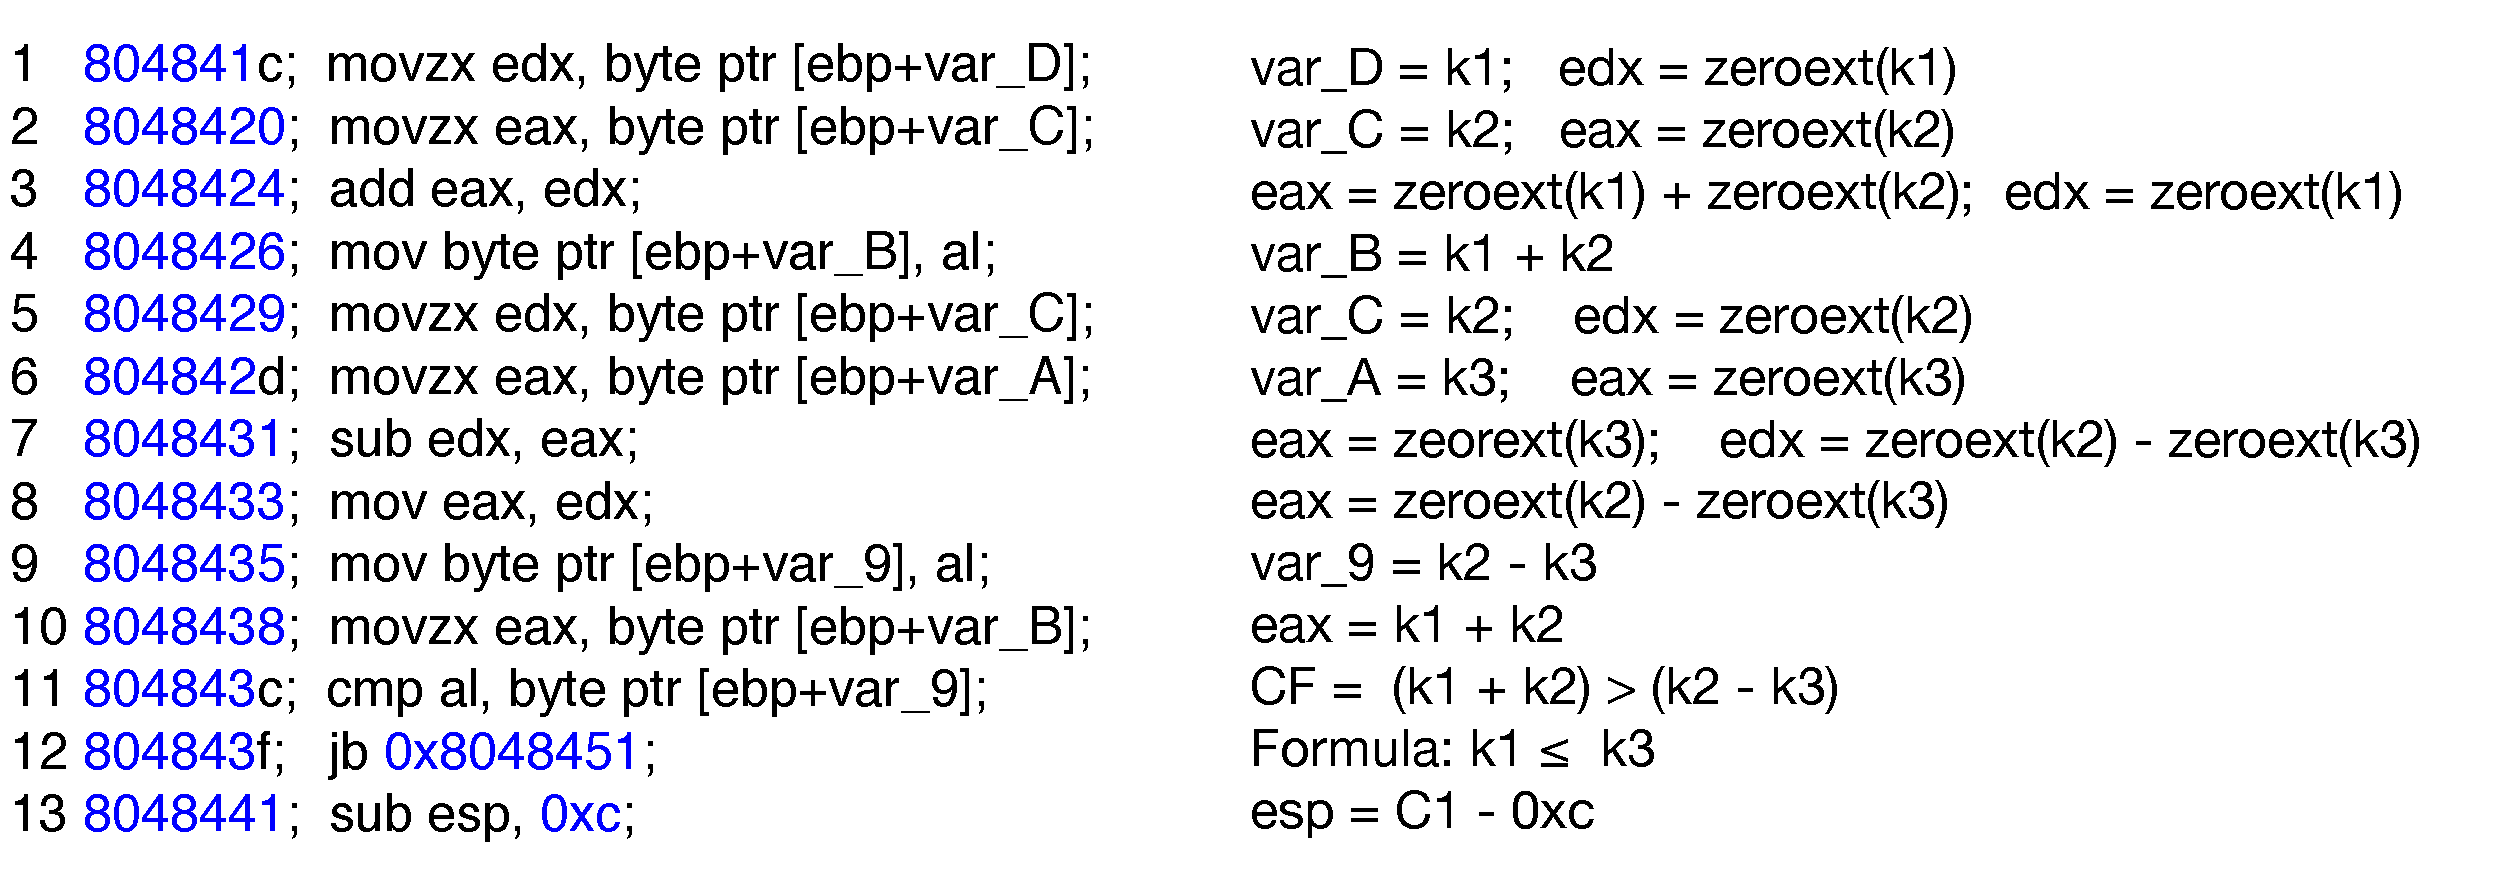
\includegraphics[width=\columnwidth]{./figures/secretCF.pdf}
      \caption{The workflow of \tool{}}
      \label{fig:Test}
  \end{figure}

For examples,

\begin{lstlisting}
...
0x0000e781      add dword [local_14h], 1
0x0000e785      cmp dword [local_14h], 4
0x0000e789      jne 0xe7df
0x0000e78b      mov dword [local_14h], 0
...
\end{lstlisting}

At the beginning of the instruction segment, the value at the 
address of local14h can be written as $F(\vec{K})$. At the address e785, 
the value will be updated with $F(\vec{K})+1$. Then the code compares 
the value with 4 and use the result as a conditional jump. 
Based on the result, we can have the following formula:

$$F(\vec{K}) + 1 = 4$$

The formula, together with the memory address (0xe789) is store
as a \textit{formula tuple (address, formula)}. 
Each formula tuple represents one leakage site.

\subsubsection{Secret-dependent data access}
Like input-dependent control-flow transfers, an adversary can also infer 
sensitive information from the data access pattern as well. 
We try to find this kind of leakages by checking 
every memory operand of the instruction. We generate the memory addressing 
formulas. As discussed before, every symbols in the formula is the input key. 
If the formula doesn’t contain any symbols, the memory access is independent 
from the input sensitive information and won’t leak any sensitive information 
according to our threat model. Otherwise, we will generate the constraint for
the memory addressing. We model the memory address with a symbolic formula 
$F(\vec{K})$. 
Because we also have the concrete value of the memory address $Addr1$. Therefore,
the formula can be written as:

$$F(\vec{K}) = Addr1$$

\subsection{Markov Chain Monte Carlo Approximate Counting}

From the above step~\ref{InstructionSE}, we can generate the constraints 
from the execution trace. 
The only variables in those constraints are the sensitive data. An adversary who 
wants to infer the sensitive data based on side-channel attacks can't observe 
the sensitive information directly. The adversary, however, can observe the
memory access pattern of the software. Each math formula can uniquely model
one leakage site.

In this section, we calculate the amount of leaked information with the
definition from~\ref{def}. The basic idea is to calculate $\frac{|K|}{|K^o|}$.
The size of $K$ is usually exponentially large. A naive method for approximating
the result is to pick $k$ elements from $K$ and check how many of them are also
contained in $K^o$. If $q$ elements are also in $K^o$. In expectation, we can
use $\frac{k}{q}$ to approximate the value of $\frac{|K|}{|K^o|}$. In this step,
we first split the contrains tuple into multiple groups depending on the memory
address. After that, we run the Markov Chain Monte Carlo to estimate the amount
of leaked information.


\subsubsection{Preprocessing}
We apply two preprocessing steps before running the Monte Carlo sampling. First,
we try to simplify those formulas by applying some normalizations rules. After
that, we split those formulas into multiple groups.

The goal of the normalization is to simplify the formulas. 
Each formulas will be evaluated multiple times with different input 
during the following sampling, 
we would like to make those formula simpler to reduce the whole execution time.  
Each formula is implemented as a abstract syntax tree. We apply a series of 
normalization rules (e.g. key1 xor key1 = 0) to simplify the formula.

After that, we split the formula tuple into multiple groups. 
Each group consists of different formulas but with the same memory address.
In other words, those formulas in the same group represent one leakage
site. The instructions inside a loop are executed multiple times with
the different item from the input buffer. We group them together to 
know the total information leakage.

The only symbol in the original formula is the key. 
An adversary who wants to infer the sensitive data based on side-channel 
attacks can't observe the sensitive information directly. 

\subsubsection{Motivation}
The adversary, however, can observe the memory access pattern of the software. 
If the attacker can observe one leakage site, the attack is modeled as one formula. 
If he observes mutiple information leakage, the attack is modeled as the conjoint 
of those formulas. Calculating the total information leakage can be reduced to the
problem of approximating the number of solutions. This is a \#P problem.

One intuition way is to use the Monte Carlo method. However, 
as the discussion in the previous section~\ref{MCreasons},
the number of satisfying keys could be exponentially small. Imagine an attacker 
who can recover one unique key after the attack, in such case, 
the conjoint of formula F = (f(k)) only has one solution.
Also, the target program may have mutiple inputs. When the number of input
symbols arises, the simple Monte Carlo may suffer from the curse of dimensionality,
which means the accuracy of the result drops dramatically when the
number of input symbols increases. 

We adopt the Markov Chain Monte Carlo (MCMC) to estimate the number of 
satisfying solutions. The basic idea is to construct a Markov Chain that
has the desired distribution.

\textit{Definition:}
Starting from here, we present the formal definition of the MCMC algorithm.
First, we introduce the definition of the concept of the algorithm.

\begin{mydef}
      An approximation scheme is an alogorithm for finding an approximation
      answer within a factor $1 + \epsilon$ of the correct number of the set
      $K^o$ with the probability of $1 - \zeta$.
\end{mydef}

\newtheorem{theorem}{Theorem}[section]

\begin{theorem}
      If $F={A_1,A_2,...,A_n}$ is a finite collection of closed sets then 
      $\cup_{i}^{n}A_i$ is a closed set.
\end{theorem}

\subsubsection{MCMC Algorithm}
In the section, we present the detail of MCMC algorithm for counting the 
cardinality of $K^o$. We will fisrt present the description of the 
MCMC and then explain the algorithm with a concrete example.
\begin{enumerate}
      \item Start with the concrete input $\vec{k} = (k_0, k_1, k_2, ..., k_n)$,
      $\vec{k}$ should be the on valid solution which satisfies the constraint
      $F = C_1(\vec{k})\land C_2(\vec{k})\land C_2(\vec{k}) \land ... \land C_m(\vec{k})$
      \item for t = 1, 2, 3,..., N
\end{enumerate}
\section{Discussions and Limitations}
In the section, we discuss \tool's limitations, usages, and some future works.

\tool{} works on the native x86 execution traces. The design, which is very
precise in terms of true leakages compared to other static source code
method~\cite{197207,BacelarAlmeida:2013:FVS:2483313.2483334}, also suffers from
limitations of dynamic approaches as well. \tool{} is not sound and has coverage
problem. Each time we only get one single execution trace. Therefore, we may
neglect some side-channel vulnerabilities on other traces. However, we argue
that it is not a crucial problems for analyzing crypto libraries. Because crypto
libraries are designed to have the same code coverage for various inputs. Our
evaluation also confirms the above point. For symmetric encryptions during our
evaluation, there is no secret-dependent control-flow transfers. RSA
implementations have several secret-dependent control-flow transfers. But after
we manually check those leakages cites. We find most of them are useful for
bound checking, which do not leak much information and have negligible effects
on the whole code coverage as well.

One of the motivations of \tool{} is that while recent works have reported lots
of tentative side-channel vulnerabilities, most of them are unpatched by
developers. Our evaluation result also confirms it. For RSA, the latest
OpenSSL\@ only has one leakage site that can leak more than 3 bits while there
are 22 leakage sites according to \tool{}. DES implementation of OpenSSL\@ has
several sensitive leakages. But given the end life status of DES, it is still
unpatched for the worth of engineering effort. At the early stage of the
project, we hope to find some sensitive leakages but are neglected by
communities for years. But somehow every sensitive leakages identified by
\tool{} are known to people before. We think the main reason is that we only
test famous crypto algorithms in well-known crypto libraries. Those code bases
have been studied for years. So it is unlikely to have unknown sensitive
leakages. We leave the task of applying \tool{} on other libraries and
non-crypto libraries in the future.

%\tool{} works on the native x86 instructions, while some existing
%works~\cite{197207,BacelarAlmeida:2013:FVS:2483313.2483334} find side-channels
%vulnerabilities from source code level or intermediate languages (e.g., VEX,
%REIL). Apart from the scalability issues for IR implementations, \tool{} is
%designed to work on the native x86 instructions for the following
%considerations. First, compliers can introduce or mitigate side channels
%vulnerabilities. For example, the GCC compiler may or may not translate the $!$
%operator into conditional branches. If the branch is secret-dependent, the
%attacker could learn some sensitive information. However, source-based methods
%fail to know how those the machine code looks like, which leads to false
%positives or false negatives.  
%Second, we find many crypto libraries have lots of inlined assembly code. In
%general, it is hard to convert assembly code into source code or IR.



\section{Implementation}
We implement the \tana\ with 12K lines of code in C++11. It has three components, one Intel
Pin tool that can collect the execution trace, the intruction-level symbolic execution
engine and the backend that can estimate the information leakage. 


\bibliographystyle{IEEEtran}
\bibliography{refs}

\end{document}


